% The ring Z[sqrt(-5)] as a lattice in the plane, with the circles of norm 2, 3, 4, 6, 9. Generated by a short script.
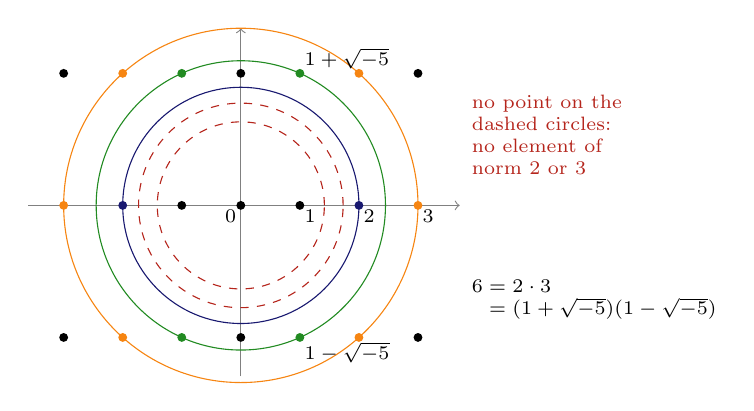
\begin{tikzpicture}
\draw[->,black!50] (-2.70,0) -- (2.78,0);
\draw[->,black!50] (0,-2.17) -- (0,2.25);
\draw[BrickRed,dashed,thin] (0,0) circle (1.061);
\draw[BrickRed,dashed,thin] (0,0) circle (1.299);
\draw[MidnightBlue,solid,thin] (0,0) circle (1.500);
\draw[ForestGreen,solid,thin] (0,0) circle (1.837);
\draw[BurntOrange,solid,thin] (0,0) circle (2.250);
\fill[black] (-2.250,-1.677) circle (1.6pt);
\fill[BurntOrange] (-2.250,0.000) circle (1.6pt);
\fill[black] (-2.250,1.677) circle (1.6pt);
\fill[BurntOrange] (-1.500,-1.677) circle (1.6pt);
\fill[MidnightBlue] (-1.500,0.000) circle (1.6pt);
\fill[BurntOrange] (-1.500,1.677) circle (1.6pt);
\fill[ForestGreen] (-0.750,-1.677) circle (1.6pt);
\fill[black] (-0.750,0.000) circle (1.6pt);
\fill[ForestGreen] (-0.750,1.677) circle (1.6pt);
\fill[black] (0.000,-1.677) circle (1.6pt);
\fill[black] (0.000,0.000) circle (1.6pt);
\node[font=\scriptsize,below left,inner sep=1.5pt] at (0.000,0.000) {$0$};
\fill[black] (0.000,1.677) circle (1.6pt);
\fill[ForestGreen] (0.750,-1.677) circle (1.6pt);
\node[font=\scriptsize,below right,inner sep=1.5pt] at (0.750,-1.677) {$1-\sqrt{-5}$};
\fill[black] (0.750,0.000) circle (1.6pt);
\node[font=\scriptsize,below right,inner sep=1.5pt] at (0.750,0.000) {$1$};
\fill[ForestGreen] (0.750,1.677) circle (1.6pt);
\node[font=\scriptsize,above right,inner sep=1.5pt] at (0.750,1.677) {$1+\sqrt{-5}$};
\fill[BurntOrange] (1.500,-1.677) circle (1.6pt);
\fill[MidnightBlue] (1.500,0.000) circle (1.6pt);
\node[font=\scriptsize,below right,inner sep=1.5pt] at (1.500,0.000) {$2$};
\fill[BurntOrange] (1.500,1.677) circle (1.6pt);
\fill[black] (2.250,-1.677) circle (1.6pt);
\fill[BurntOrange] (2.250,0.000) circle (1.6pt);
\node[font=\scriptsize,below right,inner sep=1.5pt] at (2.250,0.000) {$3$};
\fill[black] (2.250,1.677) circle (1.6pt);
\node[font=\scriptsize,BrickRed,align=left,anchor=west] at (2.81,0.90) {no point on the\\dashed circles:\\no element of\\norm $2$ or $3$};
\node[font=\scriptsize,align=left,anchor=west] at (2.81,-1.20) {$6=2\cdot3$\\$\phantom{6}=(1+\sqrt{-5})(1-\sqrt{-5})$};
\end{tikzpicture}
